%%%%%%%%%%%%%%%%%%%%%%%%%%%%%%%%%%%%%%%%%%%%%%%%%%%%%%%%%%%%%%%%%%%%%%%%
%    INSTITUTE OF PHYSICS PUBLISHING                                   %
%                                                                      %
%   `Preparing an article for publication in an Institute of Physics   %
%    Publishing journal using LaTeX'                                   %
%                                                                      %
%    LaTeX source code `ioplau2e.tex' used to generate `author         %
%    guidelines', the documentation explaining and demonstrating use   %
%    of the Institute of Physics Publishing LaTeX preprint files       %
%    `iopart.cls, iopart12.clo and iopart10.clo'.                      %
%                                                                      %
%    `ioplau2e.tex' itself uses LaTeX with `iopart.cls'                %
%                                                                      %
%%%%%%%%%%%%%%%%%%%%%%%%%%%%%%%%%%
%
%
% First we have a character check
%
% ! exclamation mark    " double quote  
% # hash                ` opening quote (grave)
% & ampersand           ' closing quote (acute)
% $ dollar              % percent       
% ( open parenthesis    ) close paren.  
% - hyphen              = equals sign
% | vertical bar        ~ tilde         
% @ at sign             _ underscore
% { open curly brace    } close curly   
% [ open square         ] close square bracket
% + plus sign           ; semi-colon    
% * asterisk            : colon
% < open angle bracket  > close angle   
% , comma               . full stop
% ? question mark       / forward slash 
% \ backslash           ^ circumflex
%
% ABCDEFGHIJKLMNOPQRSTUVWXYZ 
% abcdefghijklmnopqrstuvwxyz 
% 1234567890
%
%%%%%%%%%%%%%%%%%%%%%%%%%%%%%%%%%%%%%%%%%%%%%%%%%%%%%%%%%%%%%%%%%%%
%
\documentclass[12pt]{iopart}
\newcommand{\gguide}{{\it Preparing graphics for IOP Publishing journals}}
%Uncomment next line if AMS fonts required
%\usepackage{iopams}  
%
%% My own packages
%
\usepackage{ dsfont }
\usepackage{hyperref}
\usepackage{graphicx}
%
%% User-defined commands
%
\newcommand{\ddt}[1]{\frac{d #1}{dt}}
%\newcommand{\hmone}[1]{\|#1\|_{H^{-1}}}
\newcommand{\hmone}[1]{\|\nabla^{-1} #1\|_{L^{2}}}
\newcommand{\ltwo}[1]{\|#1\|_{L^{2}}}
%\newcommand{\hone}[1]{\|#1\|_{H^{1}}}
\newcommand{\hone}[1]{\| \nabla #1\|_{L^{2}}}
\newcommand{\htwo}[1]{\|#1\|_{H^{2}}}
\newcommand{\sint}[1]{\int_{D} #1 \, d^{d}\mathbf{x}}
\newcommand{\tint}[1]{\int_{0}^{T} #1 \, dt}
\renewcommand{\vec}[1]{\mathbf{#1}}
\newcommand{\linf}[1]{\| #1 \|_{L^{\infty}}}
\newcommand{\tavg}[1]{\langle  #1 \rangle}
\renewcommand{\u}{\mathbf{u}}
%\newcommand{\ppt}[1]{\frac{\partial #1}{\partial t}}
\newcommand{\ppt}[1]{\partial_{t} #1}
\newcommand{\lap}{\Delta }
\newcommand{\invlap}{\Delta^{-1}}
%\newcommand{\lap}{\nabla^{2}}
%\newcommand{\invlap}{\nabla^{-2}}
\newcommand{\pbrac}[1]{\left( #1 \right)}
\newcommand{\sbrac}[1]{\left[ #1 \right]}
\newtheorem{lemma}{Lemma}
\newtheorem{corollary}{Corollary}

\begin{document}

\title[Diffusion-limited mixing by incompressible flows]{Diffusion-limited mixing by incompressible flows}

\author{Christopher J. Miles$^{1,2,3}$ and Charles R. Doering$^{1,2,3}$ }

\address{$^1$ Department of Physics, University of Michigan,
Ann Arbor, MI 48104-1040, USA}
\address{$^2$ Department of Mathematics, University of Michigan,
Ann Arbor, MI 48104-1043, USA}
\address{$^3$ Center for the Study of Complex Systems, University of Michigan,
Ann Arbor, MI 48104-1107, USA}
\ead{doering@umich.edu}
\vspace{10pt}
\begin{indented}
\item[]\today
\end{indented}

\begin{abstract}
Incompressible flows can be effective mixers by appropriately advecting a passive tracer to produce small filamentation length scales. In addition, diffusion is generally perceived as beneficial to mixing due to its ability to homogenize a passive tracer. However in the case where advection and diffusion are both actively present, we provide numerical evidence that diffusion in quite general cases produce nearly neutral or even {\it negative} effects by limiting the mixing effectiveness of incompressible optimal flows. The underlying mechanism causing this limitation appears to be due to the presence of a limiting length scale given by a generalized Batchelor length \cite{Batchelor1959a}. This length scale limitation in turn affects long-term mixing rates. More specifically, we consider local-in-time flow optimisation under energy and enstrophy flow constraints with the objective of maximising mixing rate performance. We observe that, for enstrophy-bounded optimal flows, the strength of diffusion has no impact on the long-term mixing rate performance. For energy-constrained optimal flows, however an increase in the strength of diffusion decreases the mixing rate. We provide analytical lower bounds on mixing rates and length scales achievable under related constraints (point-wise bounded speed and rate-of-strain) by extending the work of Z. Lin {\it et. al.} \cite{JFM2011} and C.-C. Poon \cite{Chi-Cheu1996}. 

\end{abstract}
%
\pacs{47.85.lk, 47.85.L-, 42.10, 47.57.eb}
\ams{76R50, 37A25, 76F25, 76D55}
%
% Uncomment for keywords
\vspace{2pc}
\noindent{\it Keywords}: Mixing, incompressible flow, diffusion processes, flow control and optimisation, Batchelor scale

% Uncomment for Submitted to journal title message
\submitto{\NL}
%
% Uncomment if a separate title page is required
%\maketitle
% 
% For two-column output uncomment the next line and choose [10pt] rather than [12pt] in the \documentclass declaration
%\ioptwocol
%

\section{Introduction}

%%%%%

% 

% 

% Furthermore, we believe that the study of determining the smallest length scales achievable demands more attention. This assumption is used today throughout the computational fluid dynamics community to provide a heuristic for the grid resolutions necessary. Thus, it is important to determine what conditions on $\mathbf{u}$ are necessary to justify this assumption. 

% We explore this question and study the impact of molecular diffusion. We address this topic by considering an incompressible flow with mild physical constraints in a periodic box with side length $L$ in $d$ dimensions. We consider a mean-zero tracer concentration field $\theta$ that evolves according to the advection-diffusion equation,
%\begin{equation}
%	\label{eq:PDE_advection}
%	\ppt{\theta}+\mathbf{u}\cdot \nabla \theta=\kappa \lap\theta,
%\end{equation}
%with initial data $\theta(\mathbf{x},0)=\theta_{0}(\mathbf{x})$, where $\kappa$ is the molecular diffusion coefficient and $\mathbf{u}(\mathbf{x},t)$ is a incompressible ($\nabla\,\cdot\, \vec{u}=0$) flow field.

%%%%%

% -- Introduction of the advection-diffusion equation and inherent nonlinearities
%%% 
%%% Furthermore, the complexity of $u$ can be inherently complicated as solutions to the Navier-Stokes equations. Futhermore, when concerned with optimal mixing one must make a decision on which velocity field to  prescribe based on the the current scalar concentration field.

% -- Motivation for fluid dynamicists / physicists
%%% Impact on turbulence theory and Batchelor length.

% -- Motivation for computionational fluid dynamics practioners
%%% Impact considerations for smallest lengths in grid discretizations.

% -- Motivation for industrial process engineers
%%% Industrial processes as a motivation for studying mixing

%-- Motivation for mathematicians
%%% The approach taken here may apeal to the mathematician as an abstraction of the mixing process and focuses on the core transportation equation --- advection-diffusion. We ask how qualities (cecay of functional norms) of the solution depend on which function space $u$ belongs to. 
%%% Fundamental insights into a core partial differential equation 

%
%%-- Motivation for mathematicians
%The approach taken here may apeal to the mathematician as an abstraction of the mixing process and focuses on the core transportation equation --- advection-diffusion. We ask how qualities (cecay of functional norms) of the solution depend on which function space $\vec{u}$ belongs to. 
%%%% Fundamental insights into a core partial differential equation 
%
%By `mixing', we mean the combined influence of advection or stirring of bulk fluid motion and molecular diffusion of a tracer concentration which could take the form of temperature, salinity, solute, or any scalar quantity.
%
%of a passive tracer concentration via an incompressible fluid flow 


Mixing of a passive tracer quantity, such as temperature, solute cocentration, or salinity, by an incompressible flow is a fundamental fluid process. It is relevant to many domains such as turbulence theory \cite{Dimotakis2005,Violeau2000a}, aerospace engineering, oceanography \cite{Wunsch2004}, and atmospheric sciences. It also serves as a key industrial process within the food, pharmaceutical, petrochemical, and other industries \cite{paul2004handbook}. The estimated costs due to poor industrial mixing in 1989 was \$1 -- \$10 billion US dollars for the chemical industry alone \cite{paul2004handbook}. Although mixing is highly prevalent and used, its fundamental principles are still not fully known especially concerning how the interplay of advection and diffusion processes affect mixing rates and achievable filamentation length scales.

The effect of diffusion and advection on the rate of fluid mixing depends on the particular mixing situation characterized by the unique fluid properties, specific mixing flow, and boundary geometry. In view of the vast complexity of the mixing situation, general principles of mixing underlying these various situations would be beneficial. In particular, it is valuable to determine how the mixing rate (typically the most optimal mixing rate) depends on aggregate flow intensity measures such as energy and enstrophy. This is the objective of the research program encompassing many efforts \cite{CS2013,GI2014,JLT2012,JFM2011, Miles2017a,  JLT2012, DF2014, GM2005} in last decade. 

With these goals in mind, a common approach taken throughout the literature is to consider the evolution of a tracer quantity $\theta$ advected by an incompressible ($\nabla \cdot\vec{u}=0$) flow $\vec{u}$ with mild physical constraints within a periodic box  of side length $L$ in $d$ dimensions. The tracer concentration field $\theta$ evolves according to the advection-diffusion equation,
\begin{equation}
	\label{eq:PDE_advection}
	\ppt{\theta}+\mathbf{u}\cdot \nabla \theta=\kappa \lap\theta,
\end{equation}
with initial data $\theta(\mathbf{x},0)=\theta_{0}(\mathbf{x})$, where $\kappa$ is the molecular diffusion coefficient. The flow is constrained by enstrophy $\ltwo{\nabla\u} = \Gamma L^{d/2}$ or energy $\ltwo{\u} = UL^{d/2}$ where $\Gamma$ is the root mean square rate-of-strain and $U$ is the root mean square speed. 


The $H^{-1}$ norm or mix-norm \cite{GM2005} is also a common measure of mixing used throughout the literature and will be used here as well. For those interested in other measures of mixing, see \cite{JLT2012}. The $H^{-1}$ norm is given by  
%
\begin{equation}
\hmone{\theta}=\sqrt{\sint{ |\nabla^{-1} \theta( \vec{x},t)|^2}}=\sqrt{ \sum_{\vec{k}\neq \vec{0}} L^d \frac{|\hat{\theta}_{\vec{k}}(t)|^{2}}{|\vec{k}|^2}}
\end{equation}
%
where $\nabla^{-1}=\nabla \Delta^{-1}$, the operator $\Delta^{-1}$ acting on  a function $\rho$ returns the solution $\phi$ of the Poisson equation $ \Delta \phi = \rho $, and $\hat{\theta}_{\vec{k}}(t) =  \frac{1}{L^{d}}\sint{\theta(\vec{x},t)e^{-i\vec{k}\cdot\vec{x}}}$.  Lower values of the  $H^{-1}$ norm correspond to a more mixed state. Note that $H^{-1}$ norm can decrease in two ways. The first way is to decreasing the amplitudes of $|\hat{\theta}_{\vec{k}}|$ for $\vec{k}\neq 0$. This matches our first sense of mixing --- {\it homogenization}. The second way is by transferring spectral mass from the lower wave numbers to the higher wave numbers to take advantage of the $1/|\vec{k}|^2$ dependence. This produces a scalar field with sharp gradients and small length scales which matches our second sense of mixing --- {\it filamentation}. Thus we can see that the $H^{-1}$ embodies both senses. 

In the case without advection ($\vec{u}=\vec{0}$), equation \eref{eq:PDE_advection} reduces to the classical heat equation \cite{Evans2010}. The Fourier modes evolve according to $\hat{\theta}_{\vec{k}}(t)=\hat{\theta}_{\vec{k}}(0)e^{-\kappa|\vec{k}|^2t}$. Thus we have explicit analytical results for the decay of the $H^{-1}$ mix-norm by simply substituting this result. Note that $H^{-1}$ mix-norm will surely decay monotonically. Diffusion is incapable of transferring spectral mass from the low wave number modes to the high wave number modes and thus is incapable of filamentation. Thus the pure diffusion case solely exploits homogenization. Also notice the unequal weighting attach to each mode. The Fourier modes with large wave number $|\vec{k}|$ decay at a faster rate relative to the decay of those with small wave number.


%To further facilitate discussion, we define the following ratio as a measure of the characteristic {\it filamentation length} scale:
%\begin{equation}
%\label{eq:length}
%\lambda(t)\equiv  2\pi \frac{\|\nabla^{-1}\theta(\,\cdot\,,t)\|_{L^{2}}}{\|\theta(\,\cdot\,,t)\|_{L^{2}}}.
%\end{equation}
%Note that $\lambda(t)$ returns the wavelength of the wave number $\vec{k}$ for a tracer concentration field composed only of the Fourier mode with wave number $\vec{k}$ (i.e. $\theta(\vec{x},t) = Re[ A e^{-i\vec{k}\cdot \vec{x}}]$ where $A$ is a complex constant). In general, $\lambda$ is the weighted root mean square wavelength with weights given by $|\theta_{\vec{k}}|^2/\ltwo{\theta}^2$. 

In the case without diffusion ($\kappa = 0$), pure advection of the flow is the only method of mixing or colloquially known as stirring. For a flow that is constrained by enstrophy, the mix-norm decays at most exponentially where the exponential rate depends on the support of the initial data and is proportional to $\Gamma$ \cite{GI2014,CS2013}. This was mathematically proven by two separate approaches: G. Iyer {\it et. al.} \cite{GI2014} used regularisation results of partial differential equations \cite{Crippa} while C. Seis \cite{CS2013} used methods from optimal transportation theory \cite{villani2003topics}. Furthermore, enstrophy-constrained flows that realize this exponential decay rate have been constructed analytically \cite{Alberti2014a}. On the other hand, energy-constrained flows can achieve even faster mixing rates. In fact they can achieve {\it perfect mixing in finite time} which means that the $H^{-1}$ mix-norm approaches zero in finite time as opposed to approaching zero in infinite time as in the case for enstrophy-constrained mixing. This can be demonstrated by a `chequerboard' flow \cite{JMP2012} where the mix-norm achieves perfect mixing in finite time by a linear decay rate.  In either flow intensity constraint, note that $H^{-1}$ mix-norm decreases by exclusively exploiting filamentation without homogenization. This is  exactly opposite to the purely diffusive case.

Finally, the case with diffusion and advection is the least explored in this framework and the focus of this paper. 
It is known that the evolution of the $H^{-1}$ and $L^2$ norms decrease monotonically under the chequerboard flow introduced by \cite{JMP2012}
 while the $H^{1}$ increases until it reaches a peak and then decreases \cite{DF2014}. This peak corresponds to a  time when the length scales developed are small enough for diffusion to effectively act on steep gradients. C. Miles and C. Doering \cite{Miles2017a} explored this phenomena further in the context of a shell model, a reduced model using ordinary differential equations that mimic the spectral dynamics of the advection-diffusion equation. The authors concluded that shell-model mixing could not surpass length scales given by $\sqrt{\kappa/ \Gamma}$ for enstrophy-constrained flows and $\kappa/U$ for energy-constrained flows up to $O(1)$ constants. These length scales can be identified as a generalised Batchelor scale \cite{Batchelor1959a}, introduced in the context of turbulence theory. These limitations on the length scale in turn controlled the long-run optimal mixing rates determined to be $\Gamma$ under the enstrophy constraint and $U^2/\kappa$ under the energy constraint up to $O(1)$ constants. In contrast to the `pure' cases mentioned earlier, it is important to note that the $H^{-1}$ can now decrease by the two avenues of homogenization and filamentation simultaneously. 

At this point, we can already see a glimpse of a conflict between diffusion and advection for the ultimate goal of optimal mixing. Pure advection succeeds at filamentation by transferring spectral mass from the low wave number modes to the high wave number modes in a continuous fashion. However in the presence of diffusion, a once optimal pure advection flow exceptional at filamentation will be met with potential conflict since homogenization by diffusion may stifle its progress in progressing spectral mass to high wave number modes. Given that diffusion ubitquitous, we must come to terms with this conflict to promote more efficient mixing.

In this paper, we make progress towards answering ``What is the most optimal mixing rate in the presence of diffusion for an enstrophy or energy constrained flow?'' This question was also asked in the question of the shell model. We would like to determine if the predictions of the shell model hold in the partial differential equation setting. 

We approach the posed question by considering the general setup introduced of the evolution of passive scalar in a periodic box. We consider the local-in-time optimization problem first introduced by Z. Lin {\it et. al.} \cite{JFM2011} in the context of diffusion. Local-in-time optimization seeks to find the optimal flow that achieves the best instantaneous mixing rate. We will see that the best choice leads to a $\vec{u}$ that depends on $\theta$. This feedback causes the dynamics of $\theta$ governed by \eref{eq:PDE_advection} to be nonlinear.

%These results also imply that the filamentation length scale $\lambda$ also decays exponentially to zero over time given by the observation that the denominator of \eref{eq:length} is constant in time (this can be shown directly from \eref{eq:PDE_advection}). Since the filamentation length scale $\lambda$ is proportional $H^{-1}$ for $\kappa = 0$, we know that the $\lambda$ can become arbitrarily small as well.



%On the other hand, diffusion is generally perceived to enhance mixing rates of a passive tracer. It is a reasonable expectation since molecular diffusion of a dye can lead to a more homogeneous mixture as seen in everyday experience from allowing cream in coffee to diffusion over time without actively stirring --- diffusion surely benefits mixing in this case.  However, the case where advection and diffusion processes are both relevant with the goal of enhance mixing rates must be treated with care and is the topic of this paper. 


%We use the $H^{-1}$ norm to define the (exponential) rate of mixing as
%\begin{equation}
%\label{eq:rate}
%r(t) = -  \frac{\ddt{}\hmone{\theta}}{\hmone{\theta}}.
%\end{equation}
%The $L^{2}$ norm $\ltwo{\theta}$ and the $H^{1}$ norm $\hone{\theta}$ are also common measures of mixing and will be considered here as well. 

%In particular, we explore the impact of molecular diffusion on mixing through analytic and computational means. 
%
%
% \cite{JFM2011} showed numerical evidence that the filament width $\lambda$ seemingly decreased continually by instantaneous flow optimisation. This type of optimisation will be considered in this work as well. Self-similar flows can realise a decreasing $\lambda$ over time as shown analytically by \cite{Alberti2014a}.  It was rigorously proven independently by \cite{GI2014} and \cite{CS2013} that $\lambda$ decreased at most exponentially --- consistent with \cite{JFM2011} and \cite{Alberti2014a}. The work of \cite{GI2014} relied on PDE regularisation results of \cite{Crippa} while the approach of \cite{CS2013} used methods from optimal transportation theory \cite{villani2003topics}.
%
%For $Pe = \infty$ energy-constrained problem, \cite{JMP2012} showed that a `chequerboard' flow can also provide continually decreasing length scales. Moreover, $\lambda$ decreased at a fast enough rate to approach zero in finite time in contrast to the enstrophy-constrained problem where $\lambda$ decreases to zero in infinite time.
%
%The inclusion of diffusion ($Pe <\infty$) with the objective of optimal mixing has been explored.  \cite{DF2014} investigated optimal mixing and study the evolution of the mentioned measures ($H^{-1}, L^2,$ and $H^1$ norms) of mixing under the chequerboard flow introduced by \cite{JMP2012}. They show that the $H^{-1}$ and $L^2$ norms decrease monotonically under this flow while the $H^{1}$ increases until it reaches a peak and then decreases. This peak corresponds to a  time when the length scales developed are small enough for diffusion to effectively act on steep gradients. \cite{Miles2017a} explored this phenomena further in the context of a shell model, a reduced model using ordinary differential equations that mimic the spectral dynamics of the advection-diffusion equation. The authors concluded that shell-model mixing could not surpass length scales given by $\sqrt{\kappa/ \Gamma}$ for enstrophy-constrained flows and $\kappa/U$ for energy-constrained flows up to $O(1)$ constants. These length scales can be identified as a generalised Batchelor scale \cite{Batchelor1959a}, introduced in the context of turbulence theory. 
%

%Diffusion is generally perceived as a beneficiary to the goal of enhanced mixing rates of a passive tracer. It is a reasonable expectation since molecular diffusion of a dye can lead to a more homogeneous mixture as seen in everyday experience from allowing cream in coffee to diffusion over time without actively stirring --- diffusion surely benefits mixing in this case. However every coffee drinker knows that they can accelerate the mixing process by stirring or in other words advecting the fluid appropriately. Note that if diffusion were completely absent, then advection is the only way to enhance mixing.  Pure advection is undoubtedly beneficial in this case. However, the case where advection and diffusion processes are both relevant with the goal of enhance mixing rates must be treated with care and is the topic of this paper. 

%The length scales achievable within a passive scalar can also be affected by the same fluid properties and environmental conditions. It has
%
% 
% 

In this work, we will demonstrate that homogenization via diffusion and filamentation via advection can sometimes be in conflict and collectively produce a negative impact on mixing. We explore how diffusion impacts the evolution of the filament width $\lambda$ over time and mixing rates. We show numerical evidence that $\lambda$ appears to be limited by the Batchelor scale as seen in the shell model. Even when actively trying to choose the most optimal flow to minimise filamentation length. Thus, this may suggest that the Batchelor scale does not only limit turbulent flows but also all incompressible flows under the flow constraints considered here. Although these quantities have been known in the context of turbulence theory, the impact of these limitations on mixing rates has not been fully studied to our knowledge.


The paper is organised as follows. We introduce the necessary theory regarding local-in-time optimisation, a shell model, and $L^{\infty}$ flow constraints in section \ref{sec:theory}. Section \ref{sec:numerical_experiment} details the methodology and results of numerically implementing local-in-time flow optimisation. Lastly, we finish with a discussion and conclusion in sections \ref{sec:discussion} and \ref{sec:conclusion} respectively.



%%%
%%%
%%% THEORY
%%%
%%%


\section{Theory}
\label{sec:theory}
\subsection{Local-in-time optimisation}

We use the $H^{-1}$ norm to define the (exponential) rate of mixing as
\begin{equation}
\label{eq:rate}
r(t) = -  \frac{\ddt{}\hmone{\theta}}{\hmone{\theta}}.
\end{equation}
The $L^{2}$ norm $\ltwo{\theta}$ and the $H^{1}$ norm $\hone{\theta}$ are also common measures of mixing and will be considered here as well. 

We define the following ratio as a measure of the characteristic filamentation length scale:
\begin{equation}
\lambda(t)\equiv  2\pi \frac{\|\nabla^{-1}\theta(\,\cdot\,,t)\|_{L^{2}}}{\|\theta(\,\cdot\,,t)\|_{L^{2}}}.
\end{equation}
Note that $\lambda(t)$ returns the wavelength of the wave number $\vec{k}$ for a tracer concentration field composed only of the Fourier mode with wave number $\vec{k}$ (i.e. $\theta(\vec{x},t) = Re[ A e^{-i\vec{k}\cdot \vec{x}}]$ where $A$ is a complex constant). In general, $\lambda$ is the weighted root mean square wavelength with weights given by $|\theta_{\vec{k}}|/\ltwo{\theta}$. 


For the enstrophy-bounded flow problem, we choose the same length scale $L$, the velocity scale $L\Gamma $, and  the time scale $1/\Gamma$. For the energy-bounded flow problem, we non-dimensionalise the system by choosing $L$ as the length scale, $U$ as the velocity scale, and $L/U$ as the time scale.  Both scalings produce the following form of the advection-diffusion equation,
\begin{equation}
\label{eq:nd_ade}
	\ppt{\theta}+\mathbf{u}\cdot \nabla \theta=\frac{1}{Pe} \lap\theta,
\end{equation}
where $Pe=  \frac{\Gamma L^2}{\kappa}$ for the enstrophy-constrained case and $Pe= \frac{UL}{\kappa}$ for the energy-constrained case.   The constraints on the flow become $\ltwo{\nabla\u} = 1$ or $\ltwo{\u} = 1$.



We consider the local-in-time optimisation strategy first introduced by \cite{JFM2011} in the diffusion-less case. We find that this strategy generalises to the case with diffusion. The local-in-time optimal velocity fields maximise the instantaneous mixing rate by minimising $\ddt{}\hmone{\theta}^2$ or equivalently minimising $\ddt{\lambda^2}$ . The optimal velocity fields are given instantaneously by (in non-dimensional form)
%
\begin{equation}
\mathbf{u}= \frac{\mathds{P}(\theta \nabla \invlap\theta)}{\langle |\mathds{P}(\theta \nabla \invlap\theta)|^2\rangle^{1/2}}
\end{equation} 
%
for the energy constraint and by 
%
\begin{equation}
\mathbf{u}= \frac{-\invlap\mathds{P}(\theta \nabla \invlap\theta)}{\langle |\nabla^{-1}\mathds{P}(\theta \nabla \invlap\theta)|^2\rangle^{1/2}}
\end{equation}
%
for the enstrophy constraint where $\mathds{P}$ is the Leray divergence-free projector given by $\mathds{P}(\vec{v}) = \vec{v} - \nabla \Delta^{-1}(\nabla \cdot \vec{v})$. These flows will be studied numerically later and is the main focus of this paper.


\subsection{Shell model predictions of local-in-time optimisation}

The shell model is a reduced model of the spectral dynamics present in the advection-diffusion equation. The model consists of a system of ordinary differential equations with nearest-neighbour coupling between `shells' in wave number space. \cite{Miles2017a} performed local-in-time mixing optimisation in this model. The shell-model analysis predicts a limiting length scale given by the Batchelor scale, $\Lambda_{\Gamma} =\sqrt{\frac{\kappa}{\Gamma}}$  and its generalisation $\Lambda_{U}= \frac{U}{\kappa} $. The non-dimensional versions are given by $\lambda_{\Gamma}= \frac{1}{\sqrt{Pe}}$ and $\lambda_{U} = \frac{1}{Pe}$.  Also from here forward, we will refer to the Batchelor scale to mean either $\lambda_{\Gamma}$ or its generalisation $\lambda_{U}$.  The predicted long-term rates (after reaching the Batchelor scale) are given by $R_{\Gamma} =\kappa/\lambda_{\Gamma}^2 $  and  $R_{U}=\kappa/\lambda_{U}^2$  The non-dimensional versions are given by $r_{\Gamma} =1$ and $r_{U} = Pe $.

\subsection{Bounds for $L^{\infty}$ constrained flows}
We consider a subset of $L^{2}$ constrained flows --- those belonging to $L^{\infty}$. In this restricted setting the rate-of-strain and speed are bounded point-wise uniformly in space and time rather than demanding that they merely be $L^2$ integrable as before. We will provide bounds on $\lambda$ and measures of mixing in this restricted setting. 

\label{sec:linfty_flows}
\subsubsection{Results for $\linf{\nabla \vec{u}} = 1$}

The time derivative of $\lambda^2$ is
%
\begin{equation}
	\ddt{\lambda^2} = \frac{2}{Pe}
		\left[ 
			\frac{\hone{\theta}^2\hmone{\theta}^2}
					{\ltwo{\theta}^4}  
			- 1
		\right]
		+ 2 \frac{\sint{\nabla^{-1}\theta \cdot \nabla\vec{u} \cdot 
							\nabla^{-1}\theta  }}
					  {\ltwo{\theta}^{2}}
\end{equation}
and by H\"older's inequality, we deduce
\begin{equation}
\label{eq:length_ineq_rate-of-strain}
	\ddt{\lambda^2} \geq \frac{2}{Pe} \left[ 
			\frac{\hone{\theta}^2\hmone{\theta}^2}
					{\ltwo{\theta}^4}  
			- 1
		\right] - 2  \lambda^2 .
\end{equation}
This establishes a lower bound on $\lambda$ at each instant: by apply Gr\"onwall's inequality and the fact that the bracketed term is greater than or equal to zero, it follows that
%
\begin{equation}
\label{eq:exponential_enstrophy}
	\lambda (t) \geq \lambda(0)e^{- t}.
\end{equation}
%
Therefore, perfect mixing in finite time is impossible for bounded rate-of-strain flows.

Furthermore,
%
\numparts \begin{eqnarray}
\frac{d}{dt}\left(\frac{\|\nabla\theta\|_{L^{2}}^2}{\|\theta\|_{L^{2}}^2}\right) &= \frac{\|\theta\|_{L^{2}}^2\frac{d}{dt}\|\nabla\theta\|_{L^{2}}^2-\|\nabla\theta\|_{L^{2}}^2\frac{d}{dt}\|\theta\|_{L^{2}}^2}{\|\theta\|_{L^{2}}^4}\\
&= \frac{-2\int \partial_{i}u_{j}\partial_{i}\theta\partial_{j}\theta - \frac{2}{Pe} \|\Delta\theta\|_{L^{2}}^2}{\|\theta\|_{L^{2}}^2}+\frac{2}{Pe}\frac{\|\nabla\theta\|_{L^{2}}^4}{\|\theta\|_{L^{2}}^4} \\
&=-\frac{2}{Pe}\left(\frac{\|\Delta\theta\|_{L^{2}}^2}{\|\theta\|_{L^{2}}^2} - \frac{\|\nabla\theta\|_{L^{2}}^4}{\|\theta\|_{L^{2}}^4} \right) - 2\frac{\sint{\nabla\theta \cdot \nabla\vec{u} \cdot 
							\nabla\theta  }}{\|\theta\|_{L^{2}}^2} 
\\
&\leq 2 \frac{\hone{\theta}^2}{\ltwo{\theta}^2}
\end{eqnarray} \endnumparts
%
and using $\ddt{}\ltwo{\theta}^2 = -\frac{2}{Pe} \hone{\theta}^2$, it follows that
\begin{equation}
\ltwo{\theta}\geq  \ltwo{\theta_{0}}\exp\left[-\frac{1}{2Pe}\frac{\hone{\theta_{0}}^2}{\ltwo{\theta_{0}}^2}\left(e^{2 t} -1\right)\right].
\end{equation}
Using this with \eref{eq:exponential_enstrophy}, we deduce the lower bound
\begin{equation}
\hmone{\theta} \geq  \hmone{\theta_{0}} \exp\left[- t -\frac{1}{2 Pe}\frac{\hone{\theta_{0}}^2}{\ltwo{\theta_{0}}}\left(e^{2 t} -1\right)\right].
\end{equation}

\subsubsection{Results for $\linf{\u}= 1$}
Here we extend the result of \cite{Chi-Cheu1996} to show that the presence of diffusion rules out perfect mixing in finite time for bounded velocity flows.  First note that
%
\begin{eqnarray}
	 \hone{\theta}^2 &=& - 2\sint{\theta \lap \theta} \\
	 							&=& Pe \sint{\theta\left(\ppt{\theta}
	 									-\frac{1}{Pe}\lap \theta\right)} 
	 									-Pe \sint{\theta\left(\ppt{\theta}
	 									+\frac{1}{Pe}\lap \theta\right)},
\end{eqnarray}
%
\begin{eqnarray}
	\ddt{}\ltwo{\theta}^2 &=& 2\sint{\theta\ppt{\theta}} \\
										 &=&\sint{\theta\left(\ppt{\theta}
	 									-\frac{1}{Pe}\lap \theta\right)} 
										 + \sint{\theta\left(\ppt{\theta}
	 									+\frac{1}{Pe}\lap \theta\right)} ,
\end{eqnarray}
%
and
%
\begin{eqnarray}
	\ddt{}\hone{\theta}^2 &=& -2\sint{\ppt{\theta}\lap \theta} \\
	 									&=& Pe \sint{\left(\ppt{\theta}
	 									-\frac{1}{Pe}\lap \theta\right)^2} 
	 									-Pe \sint{\left(\ppt{\theta}
	 									+\frac{1}{Pe}\lap \theta\right)^2} .
\end{eqnarray}

Then compute:
%
\begin{eqnarray*}
	\ddt{} \pbrac{ \frac{\hone{\theta}^2}{\ltwo{\theta}^2} } 
			&=& \frac{1}{\ltwo{\theta}^4}
			\sbrac{
				\ltwo{\theta}^2\ddt{}\hone{\theta}^2
				-\ddt{}\ltwo{\theta}^2\hone{\theta}^2			
			}\\
			&=& \frac{1}{\ltwo{\theta}^4}
			\sbrac{
				\ltwo{\theta}^2
				\pbrac{
					Pe \sint{\left(\ppt{\theta}
	 									-\frac{1}{Pe}\lap \theta\right)^2} 
 					-Pe\sint{\left(\ppt{\theta}
	 									+\frac{1}{Pe}\lap \theta\right)^2} 
				}
			}\\
		&-&\frac{1}{\ltwo{\theta}^4}
			\sbrac{
				Pe
				\pbrac{
					 \sint{\theta\left(\ppt{\theta}
	 									-\frac{1}{Pe}\lap \theta\right)} 
 				}^2		
 				-
 				Pe
 				\pbrac{
					 \sint{\theta\left(\ppt{\theta}
	 									+\frac{1}{Pe}\lap \theta\right)} 
 				}^2					
			}.
\end{eqnarray*}
%
Using H\"older's inequality and \eref{eq:PDE_advection}, this simplifies to
%
\begin{eqnarray*}
	\ddt{} \pbrac{ \frac{\hone{\theta}^2}{\ltwo{\theta}^2} } 
			&\leq & \frac{Pe}{\ltwo{\theta}^2}
			\sbrac{
					 \sint{(\vec{u}\cdot \nabla \theta)^2} 
			}.
\end{eqnarray*}
Again applying H\"older's inequality we have
\begin{equation}
\label{eq:k2growth_energy}
	\ddt{} 
		\pbrac{ 
			\frac{\hone{\theta}^2}{\ltwo{\theta}^2} 
		} 
		\leq  
		Pe
		\frac{\hone{\theta}^2}{\ltwo{\theta}^2} 
\end{equation}
%
and thus 
%
\begin{equation}
		\frac{\hone{\theta}}{\ltwo{\theta}} 
		\leq  
		\frac{\hone{\theta_0}}{\ltwo{\theta_0}}
		\exp{\pbrac{\frac{Pe}{2} t}}.
\end{equation}
%
The inequality $\hone{\theta}\hmone{\theta}\geq \ltwo{\theta}^2$ then ensures that
%
\begin{equation}
\label{eq:lambda_bound}
\lambda(t) \geq \frac{\ltwo{\theta_0}}{\hone{\theta_0}}\exp{\pbrac{-\frac{Pe}{2}t}}.
\end{equation}
%
Using \eref{eq:k2growth_energy} together with  $\ddt{}\ltwo{\theta}^2 = -\frac{2}{Pe} \hone{\theta}^2$ we observe that
%
\begin{equation}
\ltwo{\theta}\geq \ltwo{\theta_{0}}\exp\left[-\frac{1}{Pe^2}\frac{\hone{\theta_0}^2}{\ltwo{\theta_0}^2}\left(e^{Pe \, \, t}-1\right)\right]
\end{equation}
%
and this combined with  \eref{eq:lambda_bound} implies
%
\begin{equation}
\hmone{\theta}\geq \frac{\ltwo{\theta_{0}}^2}{\hone{\theta_0}}\exp\left[-\frac{Pe}{2} \,\, t-\frac{1}{Pe^2}\frac{\hone{\theta_0}^2}{\ltwo{\theta_0}^2}\left(e^{Pe \,\, t}-1\right)\right].
\end{equation}



%
\section{Numerical experiment: local-in-time optimisation}
\label{sec:numerical_experiment}
\subsection{Methodology}

We solve \eref{eq:nd_ade} by using a Fourier basis to represent the $512 \times 512$ discretised spatial domain with a 4th order Runge-Kutta time-stepping method. All simulation code was created in the programming language Python with package modules, pyfftw and numpy. The code repository can be found at \href{http://github.com/cjm715/lit}{ http://github.com/cjm715/lit}.


%%%
%%%
%%% RESULTS
%%%
%%%


\subsection{Results}

\begin{figure}
\includegraphics[width=\textwidth]{images/enstrophy_film}
\caption{Local-in-time optimisation with enstrophy constraint. Top filmstrip is for $Pe =\infty$ and the bottom filmstrip is $Pe=256$. Note that the grey-scale for the $Pe=\infty$ is constant in time while it is adjusted to show the tracer concentration structure in the finite $Pe$ case. }
\label{fig:enstrophy_film}
\end{figure}
%
\begin{figure}
\includegraphics[width=\textwidth]{images/energy_film}
\caption{Local-in-time optimisation with energy constraint. Top filmstrip is for $Pe = \infty$ and the bottom filmstrip is $Pe=32$. Note that the grey-scale for the $Pe=\infty$ is constant in time while it is adjusted to show the tracer concentration structure in the finite $Pe$ case. }
\label{fig:energy_film}
\end{figure}
%
\begin{figure}
\includegraphics[width=\textwidth]{images/enstrophy_norms}
\caption{$H^{-1}, L^{2},$ and $H^{1}$ norms of the concentration field under the optimal enstrophy-constrained flow.  }
\label{fig:enstrophy_norms}
\end{figure}
%
\begin{figure}
\includegraphics[width=\textwidth]{images/energy_norms}
\caption{$H^{-1}, L^{2},$ and $H^{1}$ norms of the concentration field under the optimal energy-constrained flow.}
\label{fig:energy_norms}
\end{figure}
%
\begin{figure}
\includegraphics[width=\textwidth]{images/enstrophy_length}
\caption{The left subplot shows the filament length $\lambda$ over time subject to the optimal enstrophy-constrained flow. The right subplot is the same data except scaled: $\lambda(t)/\lambda_{\Gamma} = \lambda(t)\sqrt{Pe}$.}
\label{fig:enstrophy_length}
\end{figure}
%
\begin{figure}
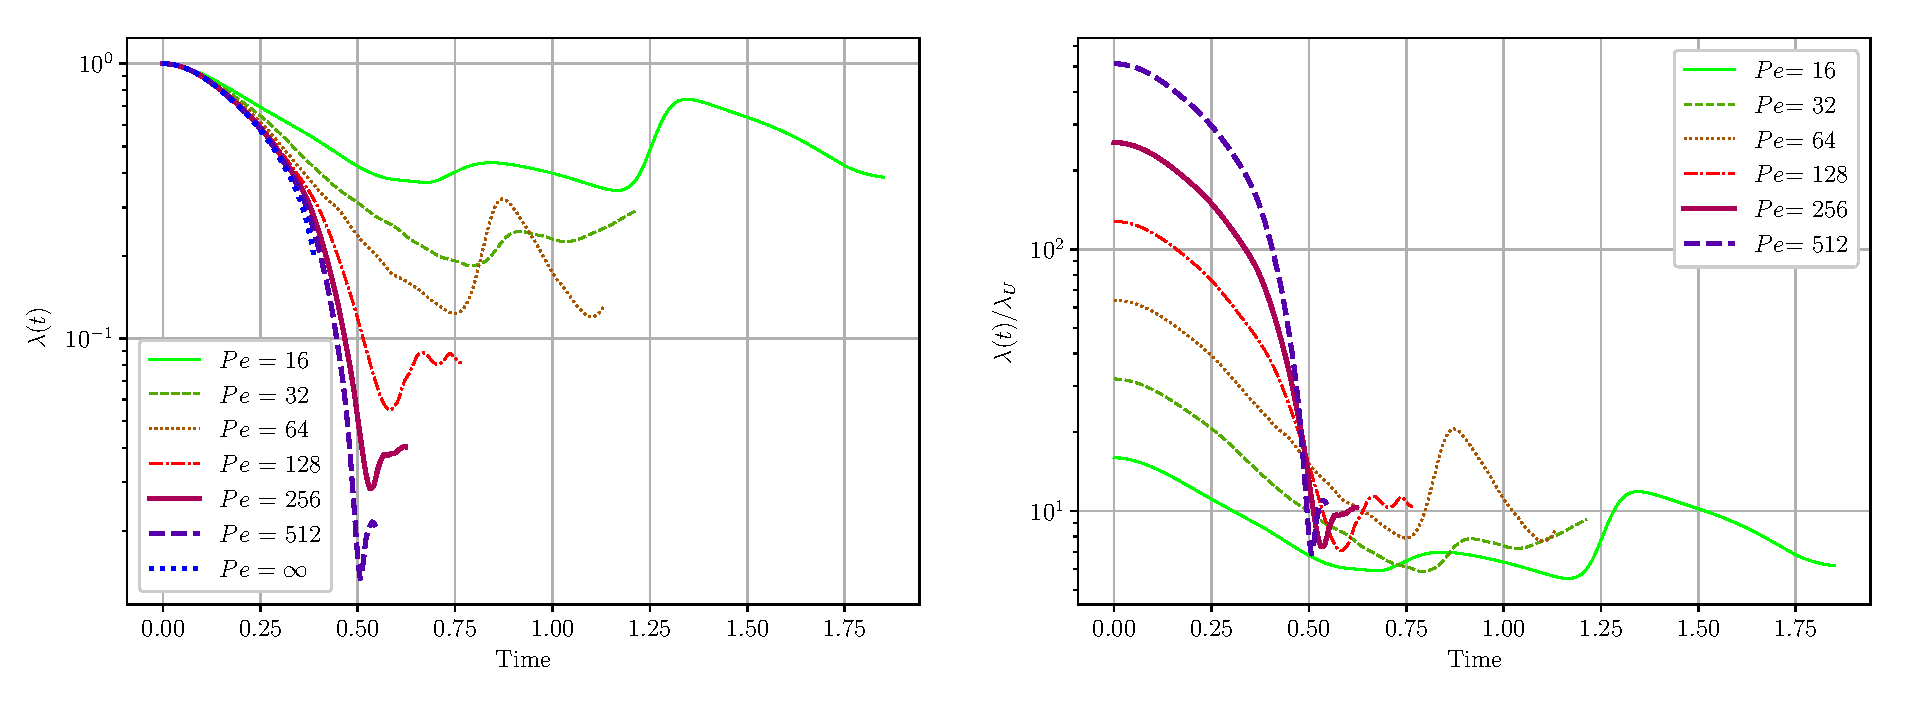
\includegraphics[width=\textwidth]{images/energy_length}
\caption{The left subplot shows the filament length $\lambda$ over time subject to the optimal energy-constrained flow. The right subplot is the same data except scaled: $\lambda(t)/\lambda_{U} = \lambda(t) Pe$.}
\label{fig:energy_length}
\end{figure}
%
\begin{figure}
\centering
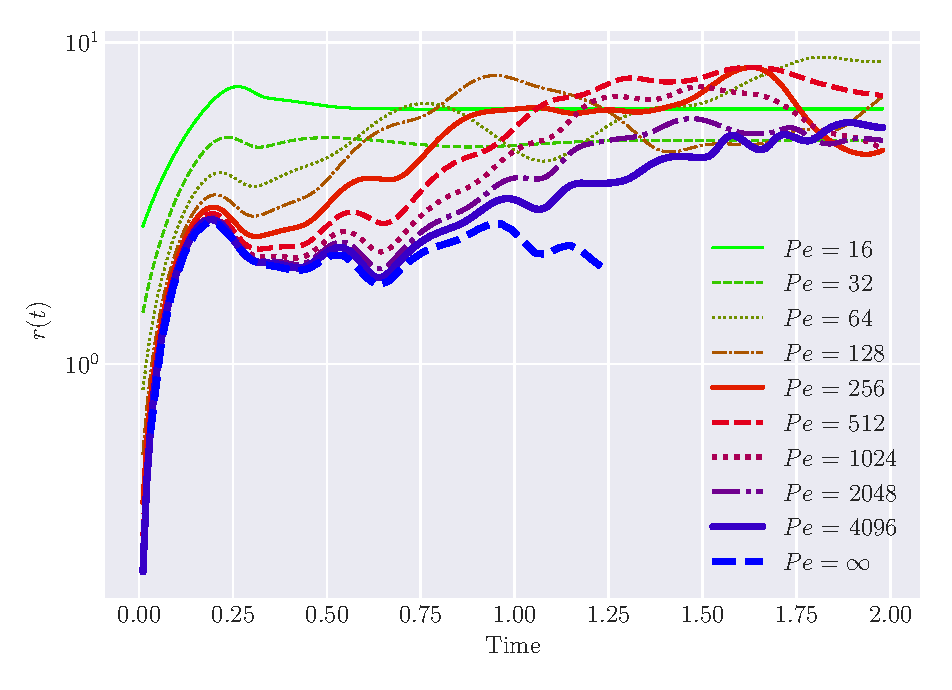
\includegraphics[width=0.5\textwidth]{images/enstrophy_rate}
\caption{Mixing rate $r(t)$ over time when subject to the optimal enstrophy-constrained flow.}
\label{fig:enstrophy_rate}
\end{figure}
%
\begin{figure}
\centering
\includegraphics[width=\textwidth]{images/energy_rate}
\caption{The left subplot shows the mixing rate $r(t)$ over time when subject to the optimal energy-constrained flow. The right subplot is the same data except scaled: $r(t)/r_{U} = r(t)/Pe$.}
\label{fig:energy_rate}
\end{figure}



 Figure \ref{fig:enstrophy_film} shows the evolution of a scalar field under the optimal flow for the enstrophy constraint. The top film strip corresponds to $Pe =\infty$ while the bottom is $Pe = 256$. The time evolution is initially similar but soon diverges over time. Figure \ref{fig:energy_film} shows the evolution for the energy case. The top film strip corresponds to $Pe =\infty$ while the bottom is $Pe = 32$. Notice that, unlike the $Pe = \infty$ cases, the flows with finite $Pe$ are incapable of creating length scales arbitrarily small for either the energy or enstrophy cases.  The left subplot of Figures \ref{fig:enstrophy_length} and \ref{fig:energy_length} shows this phenomena more quantitatively by showing $\lambda$ over time eventually reaching a plateau. The shell-model prediction of this limiting length scale is the Batchelor scale given by $\lambda_{\Gamma} = 1/\sqrt{Pe}$ for the enstrophy case and  $\lambda_{U} = 1/Pe$ for the energy case. The right plots of Figures \ref{fig:enstrophy_length} and \ref{fig:energy_length} shows scaled versions of $\lambda$ given by  $\lambda/\lambda_{\Gamma}$ and $\lambda/\lambda_{U}$ respectively.  Notice how they plateau around an $O(1)$ constant. Thus this result is consistent with the shell-model predictions. 
   
Figure \ref{fig:enstrophy_rate} shows the mixing rates for the enstrophy case. The rate during the transient phase is $\Gamma$ which is consistent with rates expected from $Pe=\infty$ mixing studies. For all $Pe$ considered, there is an increase in the rate of mixing after transient behaviour has finished to a long-term rate. Perhaps surprisingly, this long-term mixing rate appears to be {\it independent} of $Pe$ for fixed enstrophy. This suggests that the optimal long-term rate of mixing is only dependent on the rate-of-strain $\Gamma$ and not influenced by the strength of diffusion. 

Although it should be noted that the onset of the long-term rate is affected by the value of $Pe$. When there is strong diffusion (small $Pe$), the Batchelor scale is reached quickly. From the work of \cite{GI2014} and \cite{CS2013}, we know that $\lambda$ decreases at most exponentially for $Pe = \infty$. If we assume that the local-in-time optimal flows nearly saturate this bound in the transient phase, we model $\lambda$ as  $\lambda (t) = \lambda(0)\exp(- \alpha t) $ during this time. We expect the critical transition time $t_{c}$ that marks the end of this transient period to satisfy $\lambda(t_{c})= \lambda_{\Gamma}$. This time is theorised to be $t_{c}=\frac{1}{\alpha}\ln(\lambda(0)/\lambda_{\Gamma}) = \frac{1}{\alpha}\ln ( \sqrt{Pe} )$ for $Pe>1$ (If $Pe \leq 1$, then there is no transient phase). Hence, a smaller value of $Pe$ will result in an earlier onset of the long-term rate of mixing. Therefore, it is advantageous to have strong diffusion (small $Pe$) so that there is an earlier onset of the long-term mixing rate (although independent of $Pe$) which is an improvement over the mixing rate of the purely non-diffusive situation ($Pe=\infty$).
 
For the energy case, the long-term mixing rate decreases with decreasing $Pe$ (see the left subplot of figure \ref{fig:energy_rate}).  {\it Thus, strong diffusion results in a weak long-term mixing rate}. The right subplot of Figure \ref{fig:energy_rate} is $r/r_{U} =  r/Pe$. We see oscillations of $r/r_{U}$ around a value that is $O(1)$ which indicates that our numerical results are consistent with our predictions from the shell model. Thus, the long-term mixing rate is proportional to $Pe$ in contrast to the long-term mixing rate of enstrophy which carries no dependence on $Pe$.

 For the enstrophy case, we saw a benefit of picking a lower $Pe$ to result in a earlier onset of the long-term mixing behaviour. The fixed energy case however is different. The onset of the long run-mixing behaviour can be determined by the following model. From the work of \cite{JMP2012} on the fixed energy case, $\lambda(t)$ can decrease linearly in time to produce perfect mixing in finite time. We model the transient phase as $\lambda(t)=\lambda(0)(1-\beta t)$. Therefore, we theorise that the critical transition time is $t_{c}=\frac{1}{\beta}(1 -\lambda_{U}/\lambda(0)) = \frac{1}{\beta}(1 - 1/Pe)$ with $Pe> 1$ (If $Pe \leq 1$, there is no transient phase) for the energy case. Thus, it is true that on can still achieve an earlier onset of the long-term mixing behaviour by choosing a smaller $Pe$. However, an earlier onset time is accompanied by a slower long-term mixing rate. As for choosing a large $Pe$, the onset time is bounded above by $\frac{1}{\beta}$ and results in a faster long-term mixing rate. Thus, it is advantageous to have weak diffusion (large $Pe$) for mixing in the fixed energy case. This benefit is well illustrated by $H^{-1}$ norm in figure \ref{fig:energy_norms}. Notice that the mixing rate is initially slow for $Pe = 512$ but then out competes the mixing rate of smaller values of $Pe$.    

%%%
%%%
%%% DISCUSSION 
%%%
%%%

\section{Discussion}
\label{sec:discussion}
The local-in-time optimisation results suggest that there is a limiting length scale for passive tracer mixing whenever flows are optimised to decrease the mix-norm. The bounds derived under the $L^{\infty}$ constrained flow assumption did not result in proving either of these observations, but they did definitively rule out the possibility of perfect mixing in finite time for either constraint. These bounds could be drastically improved: we surmise that the deficiencies in these analyses may be due to not fully exploiting the incompressibility condition in the estimates. It remains to be shown that $\liminf_{t\rightarrow \infty} \lambda (t)\geq C\lambda_{\Gamma}$ where C is constant dependent on domain and initial condition under an enstrophy constrained flow. A similar problem remains open for the fixed energy case.  If these statements can be shown, then many of the results demonstrated here computationally will hold more generally. 

In future work, we would like to consider the optimal control problem with finite-time optimisation to minimise the filamentation width at the end time rather than instantaneously attempting to minimise its decay rate. This might lead to flows that are able to extend to even smaller length scales. Finite-time optimisation was explored in \cite{Miles2017a} in the context of the shell model where it was found that global-in-time and local-in-time optimisation appeared to give similar mixing rates. Fore the shell model, however, the analysis was consistent with computation. In the PDE case the gap between analysis and computation remains to be closed.


%%%
%%%
%%% CONCLUSION
%%%
%%%


\section{Conclusion}
\label{sec:conclusion}


Our numerical study of local-in-time optimisation suggests that there is a limiting length scale, a generalised Batchelor length scale, which in turn determines a long-term mixing ``Batchelor rate". Although the Batchelor scale has been a theorised lower bound on the length scales present on turbulent flows, it has not been shown rigorously. We hope this numerical study provides insight and promotes investigation into proving what conditions are necessary on the flow for this to be the case. Furthermore, we showed that these limitations imply that (1), for fixed enstrophy optimal flows, strong diffusion can benefit from an early onset of a long-term mixing rate (where the rate itself however is independent of diffusion strength) while (2), for energy fixed optimal flows, strong diffusion weakens the long-term mixing rate.  


\section*{Acknowledgements}
We gratefully acknowledge helpful comments from Hongjie Done, Luis Escauriaza, Guatum Iyer, Alexander Kiselev, Anna Mazzucato, Christian Seis, Ian Tobasco, and Karen Zaya. This work was supported in part by NSF Awards PHY-1205219 and DMS-1515161. One of us (CRD) is additionally grateful for Fellowship funding from the John Simon Guggenheim Memorial Foundation. 

 

\section*{References}
\bibliographystyle{iopart-num}
\bibliography{library}




\end{document}